\subsection{Bestimmung der Teilreaktionsordnung von $OH^-$}

\begin{figure}[H]
	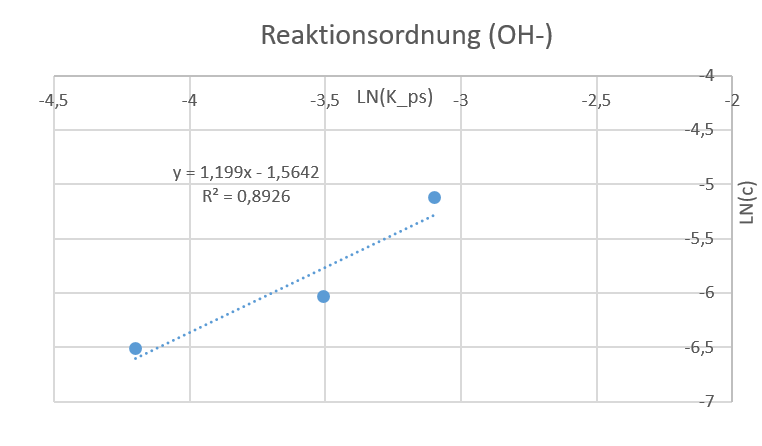
\includegraphics[width=\linewidth]{C:/Users/josefk/Desktop/kinetik/src/img/reaktionsordnung-oh.PNG}
\end{figure}

\begin{table}[H]
	\centering
	\begin{tabular}{llll}
		\toprule
		$K_{ps}$ & ln($K_{ps}$) & Konz. $OH^-$ & ln(Konz.)    \\
		\midrule
		-0,0015  & -6,502290171 & 0,015        & -4,199705078 \\
		-0,0024  & -6,032286542 & 0,03         & -3,506557897 \\
		-0,006   & -5,11599581  & 0,045        & -3,101092789 \\
		\bottomrule
	\end{tabular}
\end{table}

Die experimentell bestimmte Reaktionsordnung m ist 1,199, also 1.